\documentclass[hidelinks,12pt]{article}
\usepackage[left=0.25cm,top=1cm,right=0.25cm,bottom=1cm]{geometry}
%\usepackage[landscape]{geometry}
\textwidth = 20cm
\hoffset = -1cm
\usepackage[utf8]{inputenc}
\usepackage[spanish,es-tabla]{babel}
\usepackage[autostyle,spanish=mexican]{csquotes}
\usepackage[tbtags]{amsmath}
\usepackage{nccmath}
\usepackage{amsthm}
\usepackage{amssymb}
\usepackage{mathrsfs}
\usepackage{graphicx}
\usepackage{subfig}
\usepackage{standalone}
\usepackage[outdir=./Imagenes/]{epstopdf}
\usepackage{siunitx}
\usepackage{physics}
\usepackage{color}
\usepackage{float}
\usepackage{hyperref}
\usepackage{multicol}
%\usepackage{milista}
\usepackage{anyfontsize}
\usepackage{anysize}
%\usepackage{enumerate}
\usepackage[shortlabels]{enumitem}
\usepackage{capt-of}
\usepackage{bm}
\usepackage{relsize}
\usepackage{placeins}
\usepackage{empheq}
\usepackage{cancel}
\usepackage{wrapfig}
\usepackage[flushleft]{threeparttable}
\usepackage{makecell}
\usepackage{fancyhdr}
\usepackage{tikz}
\usepackage{bigints}
\usepackage{scalerel}
\usepackage{pgfplots}
\usepackage{pdflscape}
\pgfplotsset{compat=1.16}
\spanishdecimal{.}
\renewcommand{\baselinestretch}{1.5} 
\renewcommand\labelenumii{\theenumi.{\arabic{enumii}})}
\newcommand{\ptilde}[1]{\ensuremath{{#1}^{\prime}}}
\newcommand{\stilde}[1]{\ensuremath{{#1}^{\prime \prime}}}
\newcommand{\ttilde}[1]{\ensuremath{{#1}^{\prime \prime \prime}}}
\newcommand{\ntilde}[2]{\ensuremath{{#1}^{(#2)}}}

\newtheorem{defi}{{\it Definición}}[section]
\newtheorem{teo}{{\it Teorema}}[section]
\newtheorem{ejemplo}{{\it Ejemplo}}[section]
\newtheorem{propiedad}{{\it Propiedad}}[section]
\newtheorem{lema}{{\it Lema}}[section]
\newtheorem{cor}{Corolario}
\newtheorem{ejer}{Ejercicio}[section]

\newlist{milista}{enumerate}{2}
\setlist[milista,1]{label=\arabic*)}
\setlist[milista,2]{label=\arabic{milistai}.\arabic*)}
\newlength{\depthofsumsign}
\setlength{\depthofsumsign}{\depthof{$\sum$}}
\newcommand{\nsum}[1][1.4]{% only for \displaystyle
    \mathop{%
        \raisebox
            {-#1\depthofsumsign+1\depthofsumsign}
            {\scalebox
                {#1}
                {$\displaystyle\sum$}%
            }
    }
}
\def\scaleint#1{\vcenter{\hbox{\scaleto[3ex]{\displaystyle\int}{#1}}}}
\def\bs{\mkern-12mu}


\usepackage{titling}
\setlength{\droptitle}{-3cm}
\title{Ejercicios opcionales \\[0.3em]  \large{Material 4 - Segunda solución linealmente independiente} \vspace{-3ex}}
\author{M. en C. Gustavo Contreras Mayén}
\date{ }


\begin{document}
\vspace{-2in}
\maketitle
\fontsize{14}{14}\selectfont

\noindent

%Ref. Arfken (2006) 9.6.7
\begin{minipage}{\linewidth}
\begin{wrapfigure}{r}{0.5\textwidth}
\begin{center}
    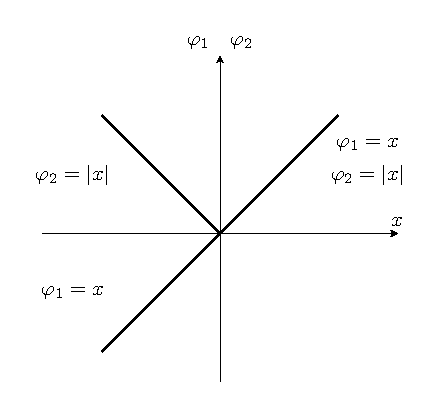
\includegraphics[width=0.5\textwidth]{Imagenes/Ejercicio_Opcional_07.eps}
\end{center}
\caption{Gráfica de las funciones $x$ y $\abs{x}$}
\label{fig:figura_09_03}
\end{wrapfigure}
\textbf{Ejercicio opcional (7). } Considera las siguientes dos funciones $\varphi_{1} = x$ y $\varphi_{2} = \abs{x} = x \, sgn \, x$, ver la figura (\ref{fig:figura_09_03}). La función $sgn x$ es el signo de $x$. Ya que $\ptilde{\varphi}_{1} = 1$ y $\ptilde{\varphi}_{2} = sng \, x$, se tiene que: $W(\varphi_{1}, \varphi_{2}) = 0$ para cualquier intervalo, incluyendo $[-1, +1]$.
\par
\noindent
Que el Wronskiano en el intervalo $[-1, +1]$: ¿prueba eso que $\varphi_{1}$ y $\varphi_{2}$ sean linealmente dependientes?. En la figura se nota claramente que no lo son. ¿Qué es lo que está mal en el argumento?
\end{minipage}
\\[1.5cm]
%Ref. Arfken (2006) 9.6.15
\textbf{Ejercicio opcional (8). } Considerando que una solución de la EDO2H:
\begin{align*}
\stilde{R} + \dfrac{1}{r} \, \ptilde{R} - \dfrac{m^{2}}{r^{2}} \, R = 0
\end{align*}
es $R = r^{m}$, demuestra que la ecuación:
\begin{align*}
\scaleint{6ex}^{x}  \, \dfrac{\exp \left[ \displaystyle - \int^{x_{2}} P(x_{1}) \dd{x_{1}} \right]}{[y_{1}(x_{2})]^{2}} \dd{x_{2}}
\end{align*}
predice una segunda solución $R = r^{-m}$.
\end{document}